\chapter{Implementation}
\label{ch:implementation}
Marty is written in Python and PL/pgSQL with a small patch to the Postgres source code written in C.
Python and PL/pgSQL are both high-level programming languages and ideal for rapid prototyping.
The source code for Marty contains two scripts, \textit{clone.py} and \textit{history.py}, which are used to create and populate the clone databases and the history database, respectively.
The patch to Postgres is necessary for Marty to be able to read the changes from the write-ahead log (WAL) with the slave instance.
It is for version 9.3.3 of Postgres and might not work with other versions.

This chapter describes the implementation of Marty.
It explains which parts of Postgres Marty uses to create the history database and keep track of the changes that are made to the master database.
It starts by explaining how the slave instance is used and why it is patched.
Next it describes the history database and its design and then continues with a description of the clone databases and how they use the history database.
The last part of this chapter describes briefly how the source code for Marty is organized.

\section{The slave instance}

\begin{wrapfigure}{r}{0.4\textwidth}
  \vspace{-20pt}
  \begin{center}
    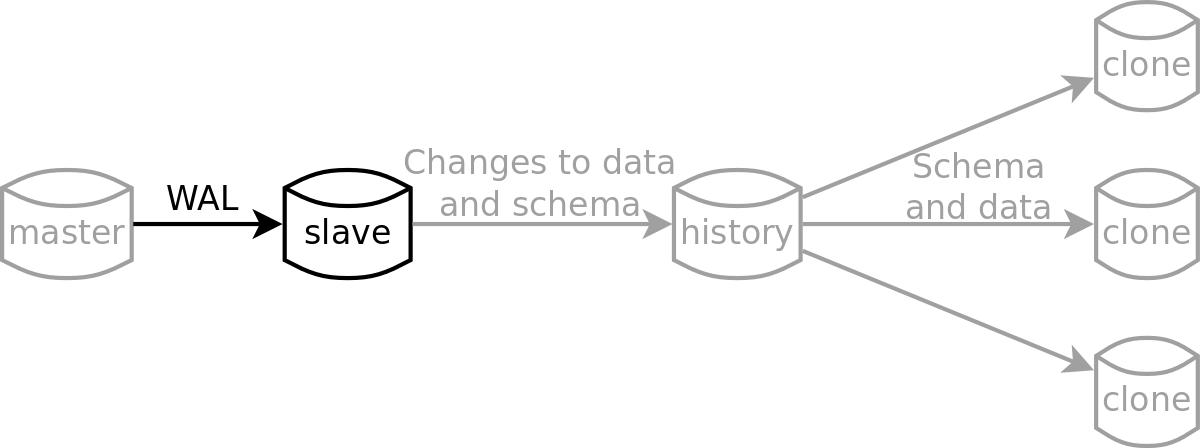
\includegraphics[width=0.38\textwidth]{img/architecture-slave}
  \end{center}
  \vspace{-20pt}
  \caption{The slave part of the architecture}
  \vspace{-10pt}
\end{wrapfigure}

Marty uses the slave instance to initialize the history database and to inspect the contents of the write-ahead log from the master.
The slave is configured to act as a \textit{hot standby} for the master; it starts with a copy of the master database and updates it with the WAL.
When the slave database is first started Marty copies its schema and data to the history database.
It then inspects the changes from the WAL as they are applied and updates the history database accordingly.

Before the slave instance is started a database administrator must configure the master.
This includes configuring a few parameters in the \textit{postgres.conf} file, see table \ref{tbl:master-config}.
Next the administrator must create a \textit{base backup} of the master database.
A base backup is a copy of the cluster files that store all the data in the database.
It can be created with the program \textit{pg\_basebackup} and might require changes to the \textit{pg\_hba.conf} file, see the Postgres documentation for further reference. % TODO add referernce?

\begin{table}[h]
  \centering
  \texttt{
    \begin{tabular}{| l | l |}
      \hline
      \textbf{Parameter} & \textbf{Value} \\ \hline
      wal\_level & hot\_standby \\ \hline
      archive\_mode & on \\ \hline
      archive\_command & 'cp \%p /path/to/archive/\%f' \\ \hline
      max\_wal\_senders & 1 \\ \hline
    \end{tabular}
  }
  \caption{Configuration parameters in postgres.conf for the master database}
  \medskip
  \small
  The archive command is an example, when the master is configured it must use an archive command that copies the WAL files to a storage where they are accessible by the slave.
  Also note that \texttt{max\_wal\_senders} must at least be 1, but can be higher.
  \label{tbl:master-config}
\end{table}

As previously noted the slave runs on a patched version of Postgres that must be compiled with a special flag that enables Postgres to log the WAL replay actions.
When the patch has been applied to the Postgres source code it must be compiled with the \texttt{WAL\_DEBUG} CPP flag.

Instead of creating a new database cluster for the slave with the \texttt{initdb} command the administrator uses the base backup from the master.
When it has been copied to the correct place the \textit{postgres.conf} file must be updated, see table \ref{tbl:slave-config}.
It is then necessary to add a \textit{recovery.conf} file with a command to fetch the WAL files from the master database, see the Postgres documentation for further reference. % TODO reference?

\begin{table}[h]
  \centering
  \texttt{
    \begin{tabular}{| l | l |}
      \hline
      \textbf{Parameter} & \textbf{Value} \\ \hline
      hot\_standby & on \\ \hline
      wal\_debug & on \\ \hline
    \end{tabular}
  }
  \caption{Configuration parameters in postgres.conf for the slave database}
  \label{tbl:slave-config}
\end{table}

\subsection{Reading the WAL}
The write-ahead log contains all the changes that are applied to the master database.
They are stored in binary records that can be applied directly to the files in the slave database cluster to repeat the changes on the slave.
There are a few different kinds of WAL records that store information about different operations on the master.
The ones that Marty looks for are \textit{heap} records and \textit{commit} records.

Heap records contain changes to the tables in the database; inserts, updates and deletes.
The commit records signal the slave to commit and close the current transaction that is being replayed from the WAL.
Other kinds of WAL records include B-tree records for B-tree indexes and XLOG records that contain information about transaction logs.

Marty can read information about the heap records in the WAL replay log.
The log contains information such as the type of the heap record; insert, update or delete, and identifiers of the database and table that the record alters.
The log also contains references to the row which was inserted, updated or deleted.

\begin{lstlisting}[caption={WAL replay log example},label={lst:wal-replay-log},numbers=left,xleftmargin=2em]
LOG:  REDO @ 0/800F1A0; LSN 0/800F248: prev 0/800F160; xid 741; len 139: Heap - insert: rel 1663/16384/11829; tid 39/63
LOG:  REDO @ 0/900390C; LSN 0/9003944: prev 0/9002158; xid 742; len 26: Heap - delete: rel 1663/16384/11829; tid 39/38 KEYS_UPDATED
LOG:  REDO @ 0/8011D80; LSN 0/8011F0C: prev 0/8011D54; xid 741; len 368: Transaction - commit: 2014-03-06 23:36:33.937958+00; inval msgs: catcache 59 catcache 58 catcache 59 catcache 58 catcache 45 catcache 44 catcache 7 catcache 6 catcache 7 catcache 6 catcache 7 catcache 6 catcache 7 catcache 6 catcache 7 catcache 6 catcache 7 catcache 6 catcache 7 catcache 6 relcache 16394
\end{lstlisting}

Listing \ref{lst:wal-replay-log} has an example of the WAL replay log.
The insert and delete heap records in lines 1 and 2 in this example alter the same table.
This table can be looked up with the \textit{rel} values in the log; 1663 is the database ID, 16384 is the namespace ID and 11829 is the table ID.
Marty uses the database and table IDs to look up the table in the slave database and queries it with the \textit{tid} values, which in this case are 39/63 and 39/38.
The tid values reference the row which was inserted to or deleted from the table.
The last line of the example, line 3, logs a commit record.
It closes the transaction and applies the changes from lines 1 and 2 to the slave database.

The next section describes the schema of the history database and how Marty queries the slave database for data to insert into the history.
\section{The history database}

\begin{wrapfigure}{r}{0.4\textwidth}
  \vspace{-20pt}
  \begin{center}
    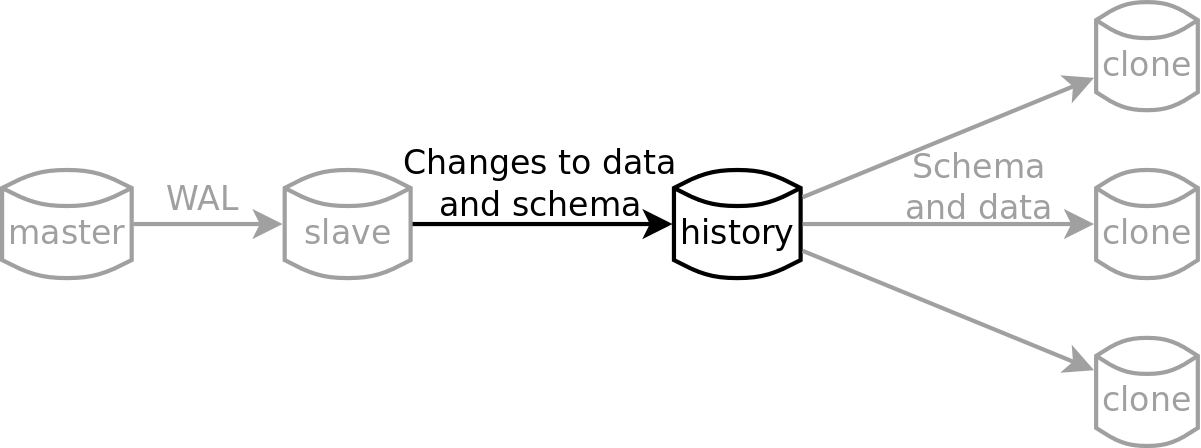
\includegraphics[width=0.38\textwidth]{img/architecture-history}
  \end{center}
  \vspace{-20pt}
  \caption{The history part of the architecture}
  \vspace{-10pt}
\end{wrapfigure}

The history database contains information about the schema of the master database and a copy of its data.
It contains multiple versions of the schema and data from the master, each transaction that alters the master database creates a history version.
It is used as a reference when the user creates a new clone database; the schema of the clone is created according to the information in the history database and its data is copied from the history.

The history database is created when the slave instance has been configured correctly.
It is a standard Postgres database that must have the same minor version as the master database.
That means that if the master runs on Postgres version 9.3.3 the history version must start with 9.3, see the Postgres documentation for further reference. % TODO add reference?

\subsection{Schema information}
To initialize the history database the administrator runs the script \textit{history.py}.
It starts by creating the \textit{schema information tables} which Marty uses to store information about the schema of the master database:

\begin{description}
  \item[marty\_schemas]
    Contains the name and ID of all schemas in the slave database.
  \item[marty\_tables]
    Contains the name and ID of the tables in the slave database and a reference to the schema they are in.
    It also stores the \textit{internal name} which is used for the data table in the history and clone databases.
  \item[marty\_columns]
    Contains the name, number, type and length of each column in the tables.
    It also stores an internal name for the column that is used in the data tables in the history and clone databases.
\end{description}

Tables \ref{tbl:marty-schemas} to \ref{tbl:marty-columns} show information about the columns of these tables.
Figure \ref{fig:schema-information-example} shows an example of their contents.

\begin{table}[h]
  \centering
  \textbf{marty\_schemas}
  \begin{tabularx}{\textwidth}{llX}
    \textit{Column} & \textit{Type} & \textit{Description} \\
    \midrule
    \_ctid & tid & A reference to the pg\_namespace table in the slave database \\
    oid & oid & The ID of the schema in the slave database \\
    name & name & The name of the schema \\
    start & integer & First version where this schema is present in the database \\
    stop & integer & First version where this schema stops being present in the database \\
  \end{tabularx}
  \caption{The columns of the marty\_schemas table}
  \label{tbl:marty-schemas}
\end{table}

\begin{table}[h]
  \centering
  \textbf{marty\_tables}
  \begin{tabularx}{\textwidth}{llX}
    \textit{Column} & \textit{Type} & \textit{Description} \\
    \midrule
    \_ctid & tid & A reference to the pg\_class table in the slave database \\
    oid & oid & The ID of the table in the slave database \\
    name & name & The name of the table \\
    schema\_oid & oid & A reference to the schema that this table belongs to \\
    internal\_name & name & The name of the data table, see chapter \ref{ch:implementation-history-data} \\
    start & integer & First version where this table is present in the database \\
    stop & integer & First version where this table stops being present in the database \\
  \end{tabularx}
  \caption{The columns of the marty\_tables table}
  \label{tbl:marty-tables}
\end{table}

\begin{table}[h]
  \centering
  \textbf{marty\_columns}
  \begin{tabularx}{\textwidth}{llX}
    \textit{Column} & \textit{Type} & \textit{Description} \\
    \midrule
    \_ctid & tid & A reference to the pg\_attribute table in the slave database \\
    table\_oid & oid & A reference to the table this column is in \\
    name & name & The name of the column \\
    number & int2 & The index of this column in the table (is it the first, second, third etc.) \\
    type & name & The type of the column (int, text, boolean etc.) \\
    internal\_name & name & The name of this column in the data table, see chapter \ref{ch:implementation-history-data} \\
    start & integer & First version where this column is part of the table \\
    stop & integer & First version where this column stops being part of the table \\
  \end{tabularx}
  \caption{The columns of the marty\_tables table}
  \label{tbl:marty-columns}
\end{table}

Postgres uses \textit{system catalogs} to store information about the schema of its databases.
They are used internally, e.g. when Postgres reads from or writes to tables.
Information such as which file in the database cluster represents which table and the column names and types of each table are stored in the system catalogs.
They are ordinary tables which are stored in a schema called \textit{pg\_catalogs} and can by queried by a user just as any other table.

Marty reads information from four system catalogs in the slave database:

\begin{description}
  \item[pg\_namespace]
    Contains information about the schemas in the slave database.
    Information from this catalog is saved in \textit{marty\_schemas} in the history database. % TODO saved in or written to?
  \item[pg\_class]
    Contains information about the tables in the slave database.
    Information from this catalog is saved in \textit{marty\_tables} in the history database.
  \item[pg\_attribute]
    Contains information about the columns of the tables in the slave database.
    Information from this catalog is saved in \textit{marty\_columns} in the history database.
  \item[pg\_type]
    Contains additional information about the columns.
    Marty reads the name of the column type from this table (integer, text etc.) and stores it in \textit{marty\_columns} along with the other column related information.
\end{description}

The history.py script creates the schema information tables and then it populates them with information about the schema of the slave database.
This is of course also the schema of the master database so the history database really contains information about the master.

Marty inspects the schema of the slave database before any WAL records have been applied to it.
It writes the schema information to the history database, which creates the first history version.
Marty then starts the WAL replay in the slave database and reads the replay log.

When a new schema is created the WAL contains an \textit{insert} heap record for the pg\_namespace table.
Marty sees this in the replay log and queries the slave about this new schema.
It then creates a new history version that includes it.
The same happens when a new table is created or a new column is added to a table; a new history version is created that includes the new table or column.

If a schema, table or column is altered, e.g. when they are renamed, the WAL has an \textit{update} heap record.
Similarly when a schema, table or column is dropped the WAL has a \textit{delete} heap record.
Marty sees this in the replay log and creates new history versions with the altered database schema.

\begin{figure}[h!]
  \centering
    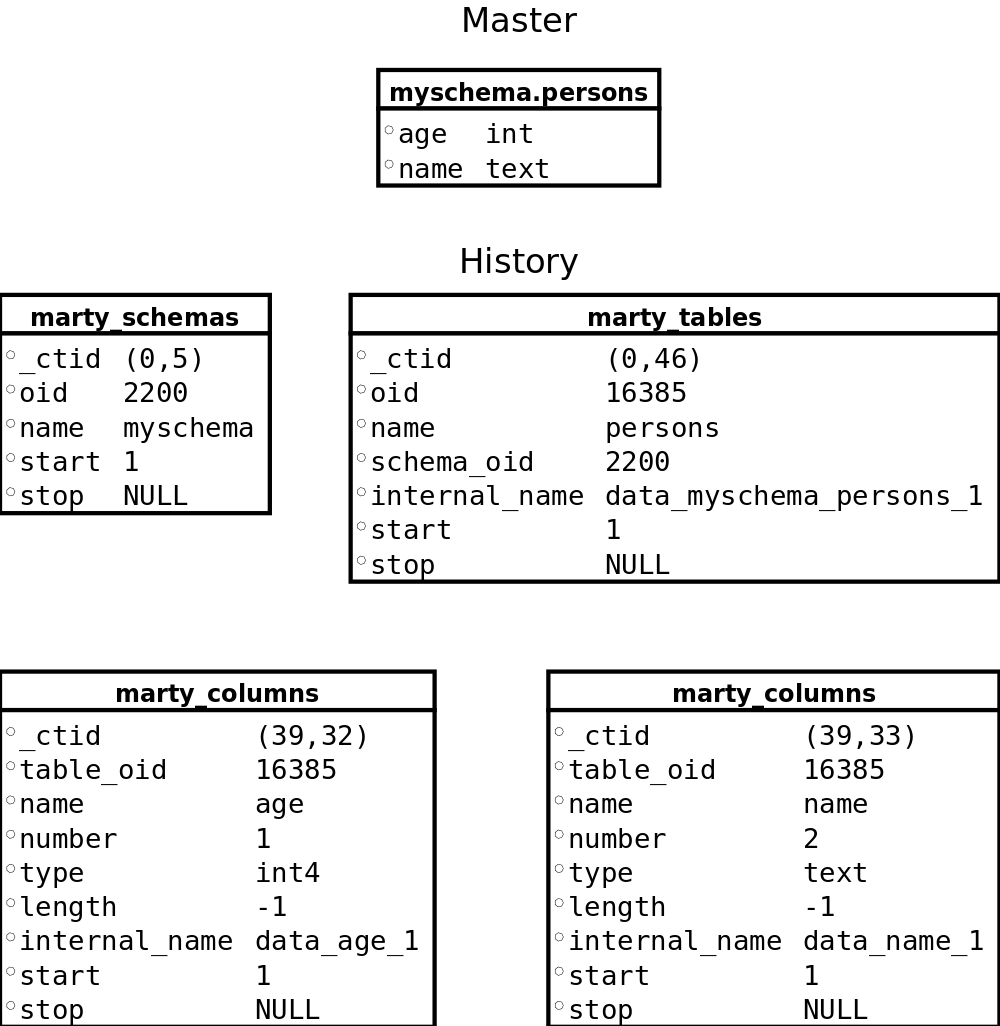
\includegraphics[width=0.75\textwidth]{schema-information-example}
  \caption{Example of the contents of the schema information tables}
  \label{fig:schema-information-example}
\end{figure}

See figure \ref{fig:schema-information-example} for an example of the contents of the schema information tables.
In the example the master database has one table, \textit{persons}, with two columns, \textit{age} of type integer and \textit{name} of type text.
The history part of the examples shows the contents of the schema information tables.

% TODO add reference to CTID and Versions subsections
\subsection{Data tables}
\label{ch:implementation-history-data}
The history database stores a copy of all the data from the slave database tables.
Marty creates a table in the history database for each table in the slave.
This happens immediately after Marty has saved the schema information about the original table to the history database.
These tables are the \textit{data tables} of the history database.

The schema of a data table is not identical to the schema of the original table.
Marty adds three columns for metadata; \textit{data\_ctid}, \textit{start} and \textit{stop}.
These columns are also present in the schema information tables (where \textit{data\_ctid} is called \textit{\_ctid}) where they serve the same purpose, see Chapters \ref{ch:implementation-history-ctid} and \ref{ch:implementation-history-versions} for more information.

When a column is added to the original table in the slave database Marty also adds it to the corresponding data table.
If a column is dropped from the original table Marty still keeps the column in the data table.
This is necessary because Marty keeps old versions of the data in the table and must therefore keep all columns that have been added to the original table, regardless of whether they have since been dropped or not.

When a row is deleted from the original table Marty marks it as deleted in the data table.
The row is still kept in the data table as part of an old history version because the data must still be accessible.
When a row is updated in the original table Marty inserts a new row into the data table with the updated values and marks the old row as deleted.
This behavior is similar to the \textit{multiversion concurrency control} (MVCC) that Postgres uses to allow more than one transaction to use the same table at the same time.

Marty does not copy any constraints from the original tables to the data tables.
The only data that the data tables contain has been copied from the original tables in the slave database.
This data conforms to the constraints of the original tables and it is therefore not necessary to replicate the constraints in the data tables.
The constraints would also cause trouble, e.g. when Marty stores updated rows from a table with a unique constraint.
If the values of the unique columns are not updated but only values in other columns then the data table could not store both the old and the new versions of the rows, as the values in the unique columns would be the same in both rows.
For these reasons Marty does not copy any constraints from the original tables.

\begin{figure}[h!]
  \centering
    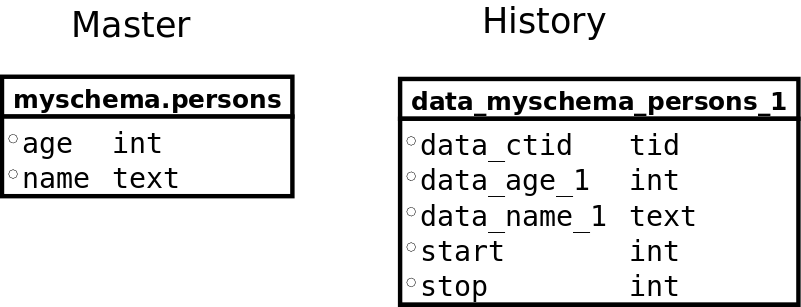
\includegraphics[width=0.6\textwidth]{history-data-table}
  \caption{An example of the schema of a data table in the history database}
  \label{fig:history-data-table-2}
\end{figure}

Marty creates all data tables in the master schema of the history database.
To avoid naming conflicts new names are creates for them: \textit{data\_[schema]\_[table]\_[version]}.
They all have the prefix \textit{data\_} followed by the name of the schema they are part of in the slave database.
Next comes the name of the original table and the name ends with the ID of the history version where this table was created.
This makes it possible for Marty to keep all the data tables in one schema in the history database, even if more than one table from different schemas share the same name in the slave database.
It also handles name reuse when a table is dropped and another table is created with the same name.
These two tables are not part of the same history version and thus the names of the data tables are different.
The columns of the data tables use similar names.
They have the \textit{data\_} prefix and are suffixed with the history version where they were added to the table.

\begin{figure}[h]
  \centering
    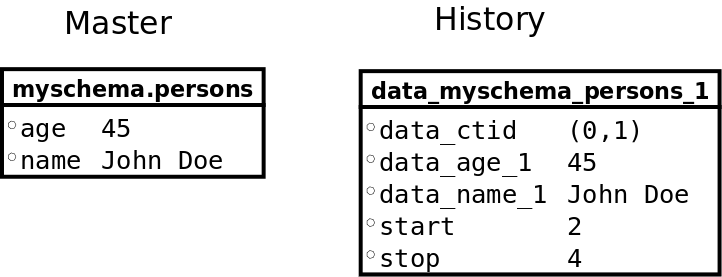
\includegraphics[width=0.6\textwidth]{history-data-table-contents}
  \caption{An example of the data in a data table in the history database}
  \label{fig:history-data-table-contents}
\end{figure}

See Figure \ref{fig:history-data-table-2} for an example of the schema of a data table in the history database.
The internal name of the data table in the history database is \textit{data\_myschema\_persons\_1}; it belongs to the schema \textit{myschema} and was created in the first history version.
It has the three metadata columns; \textit{data\_ctid}, \textit{start} and \textit{stop}.
The \textit{age} and \textit{name} columns of the original table in the master database are called \textit{data\_age\_1} and \textit{data\_name\_1} in the data table.

Figure \ref{fig:history-data-table-contents} shows an example of the contents of a data table.
The original table in the master database contains one row where age is \texttt{45} and name is \texttt{John Doe}.
This row has the ctid value of (0,1), which Marty stores in the \textit{data\_ctid} column in the data table.
It was inserted into the table in history version 2 and deleted again in history version 4.
This is reflected in the columns \textit{start} and \textit{stop}.
\subsection{CTID columns}
\label{ch:implementation-history-ctid}
The schema information tables have a column called \textit{\_ctid} and the data tables have an identical column called \textit{data\_ctid}.
The values in these columns reference the values in the \textit{ctid} columns in the corresponding tables in the slave database.
For the schema information table these are the system catalogs and for the data tables the corresponding tables are the original tables in the slave database.

The ctid column is a hidden system column that Postgres adds to all tables when they are created.
It is of type \textit{tid}, or tuple identifier, which is a pair of numbers that identify the physical location of the row inside the relation file in the database cluster.
The relation files are made up of \textit{blocks} which store the contents of the relations.
Each block contains one or more \textit{tuples} which store the actual data of the table rows.
The tuple identifier consists of a \textit{block index} and a \textit{tuple index}.
The block index is zero-based while the tuple index is one-based so the first tuple ID is (0,1).

\begin{lstlisting}[caption={WAL update and delete example},label={lst:wal-update-delete},numbers=left,xleftmargin=2em]
LOG:  REDO @ 0/60080CC; LSN 0/6008198: prev 0/600806C; xid 735; len 37; bkpb0: Heap - update: rel 1663/16384/16385; tid 0/1 xmax 735 ; new tid 0/2 xmax 0
LOG:  REDO @ 0/600822C; LSN 0/6008264: prev 0/6008204; xid 737; len 26: Heap - delete: rel 1663/16384/16385; tid 0/3 KEYS_UPDATED
\end{lstlisting}

The values in the ctid column can be used to identify each row in the database.
Marty saves this value in the schema information tables and data tables to be able to identify deleted and updated rows.
The WAL replay log from the slave instance contains the tuple identifier of the rows that are updated or deleted in the WAL records.
Marty uses the tid value to locate the correct row in the schema information tables or data tables in the history database and marks these rows as deleted.
See Listing \ref{lst:wal-update-delete} for an example.
In the example the update record in the first line inserts a new row with tid value of (0,2) to replace the old values in row with tid value of (0,1).
The delete record in the second line deletes a row with tid value of (0,3).

Note that the value of the ctid column can change, e.g. when Postgres \textit{vacuums} the table or when a row is updated.
Therefore it is not a viable long-term key to identify the row.
This does not affect the way Marty uses it because it only needs to know the tid value of the row until it changes.
When it is changed in the slave database Marty reflects this change in the history database and saves the new tid value.

Figure \ref{fig:schema-information-example} shows an example of the values in the \textit{\_ctid} column in the schema information tables.
The table \textit{marty\_schemas} contains information that Marty reads from the \textit{pg\_namespace} system catalog.
In the example this table contains one row with values from the row with ctid (0,5) in \textit{pg\_namespace}.
The table \textit{marty\_tables} contains one row with information from the \textit{pg\_class} system catalog.
It contains values from the row with ctid (0,46) in \textit{pg\_class}.
The table \textit{marty\_columns} contains two rows with information from the \textit{pg\_attribute} catalog.
They contain values from the rows with ctids (39,32) and (39,33) in \textit{pg\_attribute}.

Figure \ref{fig:history-data-table-contents} shows an example of a value in the \textit{data\_ctid} column in a data table.
The data table is called \textit{data\_myschema\_persons\_1} and the row it contains has values from a row in the original table in the master database that has the ctid value (0,1).
\subsection{History versions}
\label{chapter:implementation-history-versions}
\clearpage
\section{The clone databases}
\label{ch:impementation-clones}

\begin{wrapfigure}{r}{0.55\textwidth}
  \vspace{-20pt}
  \begin{center}
    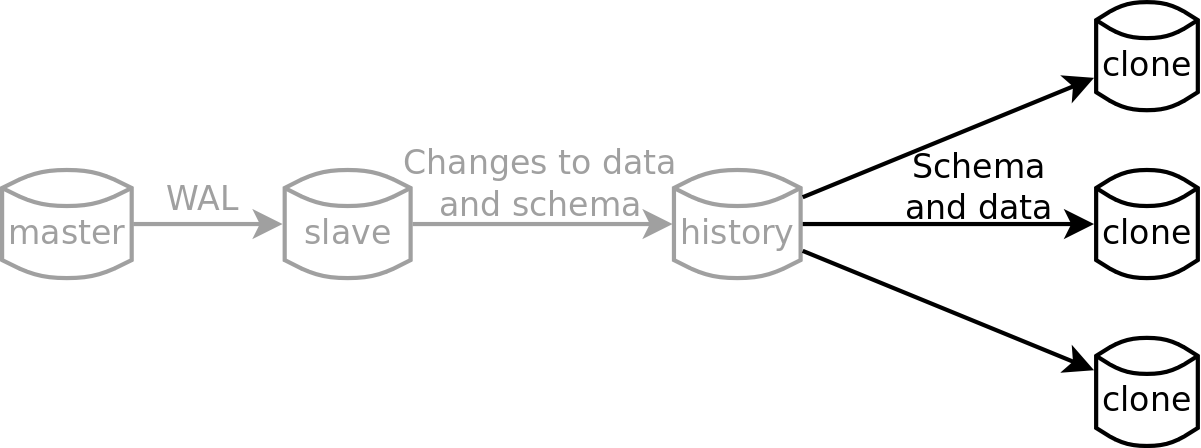
\includegraphics[width=0.53\textwidth]{img/architecture-clones}
  \end{center}
  \vspace{-20pt}
  \caption{The clone part of the architecture}
  \vspace{-10pt}
\end{wrapfigure}

A clone database is a replica of the master database.
The user can query the clone just like she would query the master.
It is a standard Postgres database that uses the \textit{PL/pgSQL} and \textit{dblink} extensions.
The user creates a new, empty database and runs the script \textit{clone.py} to initialize it as a clone.
The script reads the schema information from the history database and initializes the clone accordingly.

Like the history database the clone database must have the same major version as the master.
If the master has the version 9.3.3 that means that the clone databases must have a version number that starts with 9.3.

The initialization script creates schemas in the clone database to match those in the master database.
The tables in the clone are lazy-loading.
This means that a table is empty until a user queries it for the first time.
The clone then fetches its content from the history database.
This is implemented with a view which the user queries and an accompanying data table which stores the data once it has been fetched from the history.

The data tables live in a schema called \textit{marty}.
They have the same name as the data tables in the history database (see Chapter \ref{ch:implementation-history-data}).
The columns are identical to the columns in the original table in the master database, there are no extra columns and their names are identical to the column names in the original table.
See Figure \ref{fig:clone-tables-2} for an example of a data table.

\begin{figure}[h!]
  \centering
    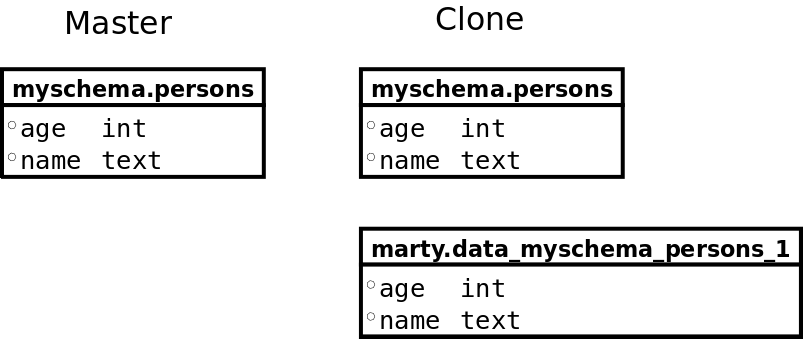
\includegraphics[width=0.6\textwidth]{clone-tables}
  \caption{Table layout in a clone database}
  \medskip
  \small
  The table \textit{persons} is actually a view that returns results from the table \textit{data\_myschema\_persons\_1} which is in the \textit{marty} schema.
  \label{fig:clone-tables-2}
\end{figure}

When the user queries a table in the clone database like she would query it in the master she is actually querying the view that Marty creates.
It executes a PL/pgSQL function, \textit{view\_select}, which returns the contents of the original table in the master.
The function is created by Marty when the clone is initialized.
It receives one argument, the name of the view that is being queried, and fetches the data for it from the corresponding data table.
When the view is queried for the first time the view\_select function fetches the data from the history database and inserts it into the data table before returning the results.
See Listing \ref{lst:view-select} for the source code of the view\_select function.

\lstset{
  language=SQL,
  morekeywords={
    FUNCTION, RETURNS, SETOF, RECORD, DECLARE, BEGIN,
    IF, RAISE, NOTICE, RETURN, QUERY, LANGUAGE,
    int, text
  }
}
\begin{lstlisting}[caption={The view\_select function},label={lst:view-select},numbers=left,xleftmargin=2em]
CREATE FUNCTION view_select(my_view_name text) RETURNS SETOF RECORD AS $$
DECLARE
  view_info RECORD;
BEGIN
  SELECT * FROM marty.bookkeeping WHERE view_name = my_view_name INTO view_info;
  IF NOT view_info.cached THEN
    RAISE NOTICE 'fetching %', view_info.view_name;
    EXECUTE ' INSERT INTO ' || view_info.local_table ||
      ' SELECT ' || view_info.coldef ||
      ' FROM dblink(''' || coninfo() || ''', ''' || view_info.remote_select_stmt || ''')'
      ' AS ' || view_info.temp_table_def;
	UPDATE marty.bookkeeping SET cached = true WHERE view_name = my_view_name;
  END IF;
  RETURN QUERY EXECUTE 'SELECT ' || view_info.coldef || ' FROM ' || view_info.local_table;
END;
$$ LANGUAGE plpgsql;
\end{lstlisting}

Marty keeps track of which data tables have been populated in the table \textit{bookkeeping}.
It is created alongside the data tables in the marty schema when the clone database is initialized and is used to store information about the data tables and views.
It stores which data table keeps the data for which view and whether it has been initialized, as well as information about how to query the history database to fetch the data for each view.
See Table \ref{tbl:bookkeeping} for a list of columns in the bookkeeping table.

\begin{table}[h]
  \centering
  \textbf{bookkeeping}
  \begin{tabularx}{\textwidth}{llX}
    \textit{Column} & \textit{Type} & \textit{Description} \\
    \midrule
    view\_name & name & The name of the view \\
    local\_table & name & The name of the data table that contains the data for the view \\
    cached & boolean & True if the data table has been populated with data from the history database \\
    coldef & text & A list of columns in the data table, used by the \textit{view\_select} function when querying the data table \\
    remote\_select\_stmt & text & The select statement for the data table in the history database \\
    temp\_table\_def & text & Table definition for a temporary table, used by view\_select \\
  \end{tabularx}
  \caption{The columns of the bookkeeping table}
  \label{tbl:bookkeeping}
\end{table}

The \textit{cached} column is a boolean which tells the view\_select function whether the data table has been populated with data from the history database (line 6 in Listing \ref{lst:view-select}).
It defaults to false as all data tables start empty.
The function uses the \textit{coldef} value when it queries the data table.
It is a comma separated list of the columns in the data table and is used to construct the select query (line 14).
When the view\_select function queries the history database it uses the \textit{remote\_select\_stmt} as the query (lines 7 to 11).
It is a select query that returns all rows from the data table in the history.
The \textit{dblink} function from the dblink extension is used to query the history database (line 10).
It receives two parameters; a connection string and the query to run.

The connection string is generated when the clone database is initialized.
Marty creates a function, \textit{coninfo}, that returns this string.
This makes it simple to update the connection string later in a running clone database if the setup of the history database changes, as only this one-line function needs to be redefined instead of the whole view\_select function.
The query that returns the data from the history database is created when Marty initializes the clone and is saved in the \textit{remote\_select\_stmt} column in the bookkeeping table.


\begin{lstlisting}[caption={An example of a SELECT query with a table alias},label={lst:table-alias-query}]
SELECT * FROM dblink('dbname=mydb', 'SELECT age, name FROM persons') AS p(age int, name text)
\end{lstlisting}

The dblink query must have an alias part where the names and types of the columns in the result rows are specified.
This is because the dblink function is declared to return a set of \textit{records}.
Postgres does not know the format of the records so the user must provide this information with the alias\footnote{http://www.postgresql.org/docs/9.3/static/contrib-dblink-function.html}.
See Listing \ref{lst:table-alias-query} for an example.
The part after \textit{AS} tells Postgres what to expect in the query results.
This part is unique to each data table in the clone database.
It is saved in the \textit{temp\_table\_def} column in the bookkeeping table and is appended to the dblink query in the view\_select function (line 11).
\section{Source code}
The source code for Marty contains two Python scripts that can be run from the command line.
Those are \textit{history.py}, which a database administrator uses to initialize the history database, and \textit{clone.py} which a user runs to initialize a clone database.
The rest of the code consists of three Python files which contain classes that the scripts use.

\begin{description}
  \item[inspector.py]
    Contains the classes \textit{SlaveInspector} and \textit{HistoryInspector}.
    The SlaveInspector is used by history.py to gather information about the schemas and tables in the slave database.
    The HistoryInspector is used by clone.py to read the schema and table information from the history database.
  \item[populator.py]
    Contains the classes \textit{HistoryPopulator} and \textit{ClonePopulator}.
    The HistoryPopulator is used by history.py to insert the information from the SlaveInspector into the history database.
    The ClonePopulator is used by clone.py to create schemas and tables in the clone database according to the information from the HistoryInspector.
  \item[dbobjects.py]
    This file contains a few classes that the inspectors use to supply the populators with data.
    They include \textit{Schema}, \textit{Table} and \textit{Column} which contain the name and other data about each one of those objects.
    The Table and Column classes also have methods to create the names of the data tables and its columns.
\end{description}

The history.py script receives ten arguments:

\texttt{---slave-host} The hostname or IP address of the slave database \\
\texttt{---slave-port} The port number of the slave database \\
\texttt{---slave-user} The username for the slave database \\
\texttt{---slave-password} The password for the slave database \\
\texttt{---slave-database} The name of the slave database \\
\texttt{---history-host} The hostname or IP address of the history database \\
\texttt{---history-port} The port number of the history database \\
\texttt{---history-user} The username for the history database \\
\texttt{---history-password} The password for the history database \\
\texttt{---history-database} The name of the history database

The clone.py script receives the same arguments for the history database and similar arguments for the clone database that should be initialized.

The clone.py script only uses the data in the history database to populate the clone.
The history.py script receives the WAL replay log from the slave database as standard input.
It uses a couple of classes to consume and parse the log, \textit{Worker} and \textit{RegExer}.
The Worker class reads the log and keeps a list of all heap records it encounters.
When it reads a commit record it creates a new history version in the history database and runs through the heap records, saving the changes to the new history version.
To parse the log records it uses the RegExer class, which is a wrapper around regular expressions which are used to match and extract data from the replay log.
See chapter \ref{ch:reading-the-wal} for an explanation of the WAL replay log, heap records and commit records.

All SQL and PL/pgSQL code in Marty is part of the Python scripts.
Marty is not a large project and the current version contains a little under 1100 lines of code.
Included in that number is the file that contains the patch to the Postgres source code.

% TODO add a reference to the souce code in the Appendix